%!TEX program=xelatex
\documentclass[a4paper]{article}
\usepackage{ctex}
\usepackage{geometry}
\usepackage{multirow}
\usepackage{tabularx}
\usepackage{float}
\usepackage{graphicx}
\usepackage{diagbox}

\geometry{left=3.0cm,right=3.0cm,top=3.5cm,bottom=3.5cm}

\title{同轴电缆中电磁波的传输和金属中超声波的传输}
\author{2017011341, 陈旭}
\date{2019 年 4 月}

\begin{document}

\maketitle

\section{同轴电缆中电磁波的传输}

    \subsection{实验目的}

        \par 通过脉冲波信号的测量,理解波在传输路径上遇到界面时的反射和透射特性,理解入射波和反射波的相位关系,掌握阻抗匹配概念。

    \subsection{实验原理}

        \par 设传输线长为 $l$,在终端 $z=l$ 处外加负载 $Z_l$,可得 $\Gamma=\frac{Z_l-Z_0}{Z_l+Z_0}=|\Gamma|e^{j\theta}$。外加不同负载时参数如下:

        \begin{itemize}
            \item 开路:$Z_l=R_l=\infty$,$\Gamma = 1$;
            \item 短路:$Z_l=R_l=0$,$\Gamma = -1$;
            \item 负载匹配:$Z_l=R_l=R_0$,$\Gamma = 0$。
        \end{itemize}
    
    \subsection{实验任务}

        \par 测量同轴电缆的长度和衰减常数,分析传输线终端反射波和入射波的相位关系。测量长度时:
        \begin{itemize}
            \item 将信号发生器输出信号通过电阻盒接到传输线“输入端”,选择合适的脉冲。
            \item 传输线“输出端”分别选择开路、短路和匹配电阻三种测试方式。利用示波器分别测出传输线“输入端”、“输出端”之间信号波形和相对延时。
            \item 分别利用测量结果计算同轴电缆的长度,并估算不确定度。
            
        \end{itemize}

    \subsection{数据处理}
    
        \subsubsection{开路负载}

            \begin{table}[H]
                \centering
                \begin{tabular}{|c|c|c|c|c|c|c|}
                    \hline
                                    & 1         & 2         & 3         & 4         & 5         & 6         \\ \hline
                    $V_i\ (mV)$     & 500       & 428       & 340       & 268       & 212       & 164       \\ \hline
                    $\tau_i\ (ns)$  & 120       & 250       & 390       & 530       & 660       & 800       \\ \hline
                    $\ln{V_i}$      & 6.2146    & 6.0591    & 5.8289    & 5.5910    & 5.3566    & 5.0999    \\ \hline
                \end{tabular}
                \caption{开路负载下实验数据记录}
            \end{table}

            \par 对 $\ln{V_i}$ 进行直线拟合,得:

            \begin{figure}[H]
                \centering
                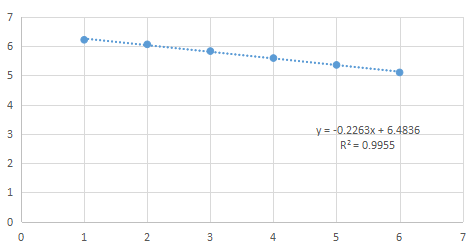
\includegraphics[width=0.7\linewidth]{figures/f1}
                \caption{$\ln{V_i}$ 直线拟合结果}
            \end{figure}

            \par 根据 $V_l=Ve^{-\alpha l}$,得 $\alpha l=0.2263$。

            \par 再对 $\tau_i$ 进行直线拟合,得:

            \begin{figure}[H]
                \centering
                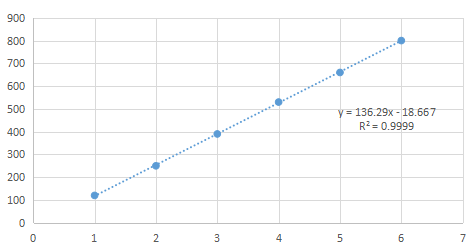
\includegraphics[width=0.7\linewidth]{figures/f2}
                \caption{$\tau_i$ 直线拟合结果}
            \end{figure}

            \par 根据 $\tau_i=i\cdot l/u$,得 $t=\tau_1=136.29 ns$。

            \par 所以,电缆长度为 $l=ut=27.26m$,$\alpha=\frac{\alpha l}{l}=8.302\times 10^{-3}m^{-1}$。

            \par 因为 $\Delta_B=25ns$,$\Delta_A=\tau_1\cdot t_p(4)\sqrt{\frac{R^{-2}-1}{6-2}}=1.8945ns$,

            \par 所以 $\Delta_l=u\Delta_t=u\cdot\sqrt{\Delta^2_A+\Delta^2_B}=5.01m$。

            \par 综上所述,$\alpha=8.302\times 10^{-3}m^{-1}$,$l=(27.26\pm5.01)m$。

        \subsubsection{短路负载}

            \begin{table}[H]
                \centering
                \begin{tabular}{|c|c|c|c|c|c|c|}
                    \hline
                                    & 2         & 4         & 6         \\ \hline
                    $V_i\ (mV)$     & 400       & 264       & 168       \\ \hline
                    $\tau_i\ (ns)$  & 240       & 500       & 760       \\ \hline
                \end{tabular}
                \caption{短路负载下实验数据记录}
            \end{table}

            \par 由实验数据取平均值得 $t_2=\frac{1}{3}\cdot(\tau_2+\tau_4/2+\tau_6/3)=247.78ns$,$S_{\tau}=5.666$。

            \par 所以,电缆长度为 $l=ut_2/2=24.78m$。

            \par 因为 $\Delta_B=25ns$,$\Delta_A=t_p(2)S_{\tau}/\sqrt{n}=14.065ns$,

            \par 所以 $\Delta_l=u\Delta_t/2=u\cdot\sqrt{\Delta^2_A+\Delta^2_B}/2=2.87m$,$l=(24.78\pm2.87)m$。

        \subsubsection{匹配负载}

            \begin{table}[H]
                \centering
                \begin{tabular}{|c|c|c|c|c|c|c|}
                    \hline
                                    & 1         & 1         & 1         \\ \hline
                    $\tau_i\ (ns)$  & 120       & 120       & 120       \\ \hline
                \end{tabular}
                \caption{匹配负载下实验数据记录}
            \end{table}

            \par 由实验数据取平均值得 $t_1=120ns$。

            \par 所以,电缆长度为 $l=ut=24.00m$。
        
\section{金属中超声波的传输}
    
    \subsection{实验目的}

        \par 掌握超声波波速测量方法,观察声波转换及表面波,了解超声波来探测原理。
    
    \subsection{实验任务}

        \par 先将超声试验仪上“发射/接收”连接端与超声探头相连接,“检波”连接示波器作为输出。调整衰减器,使输出波形最适用。

        \begin{itemize}
            \item 测量声速:采用脉冲波反射法,计算公式:$c=\frac{2l}{t_2-t_1}$。分别使用直探头和斜探头测量纵波声速和横波声速,计算样品的杨氏模量和泊松系数。
            \item 表面波实验:根据表面波在传播中遇到尖锐界面后反射回波的特性,测定起始表面波脉冲与回波脉冲的时间间隔以及传播距离,即可测出表面波的波速。
            \item 超声波探测缺陷:使用斜探头测量,利用超声波在材料中传播的距离来计算缺陷位置。
        \end{itemize}
    
    \subsection{数据处理}

        \subsubsection{横、纵波声速}

            \begin{table}[H]
                \centering
                \begin{tabular}{|c|c|c|c|c|c|c|}
                    \hline
                                        & 1         & 2         & 3         \\ \hline
                    $t_H-t_1\ (\mu s)$  & 19.4      & 19.0      & 19.2      \\ \hline
                \end{tabular}
                \caption{纵波测量实验数据记录}
            \end{table}

            \par 由实验数据取平均值得 $t=t_H-t_1=19.2\mu s$,$S_t=0.1633$。

            \par 所以,纵波声速为 $c_l=2l/t=6260.417m/s$。

            \par 因为 $\Delta_B=0.5\mu s$,$\Delta_A=t_p(2)S_{\tau}/\sqrt{n}=0.4054\mu s$,

            \par 所以 $\Delta_t=\sqrt{\Delta^2_A+\Delta^2_B}=0.6437\mu s$,$\Delta_{c_l}=c_l\times\sqrt{(\frac{\Delta_l}{l})^2+(\frac{\Delta_t}{t})^2}=209.899m/s$。

            \par 所以 $c_l=(6.260\pm 0.209)\times 10^3m/s$。

            \begin{table}[H]
                \centering
                \begin{tabular}{|c|c|c|c|c|c|c|}
                    \hline
                                        & 1         & 2         & 3         \\ \hline
                    $t_{R_2}-t_{R_1}\ (\mu s)$  & 19.2      & 19.2      & 19.6      \\ \hline
                \end{tabular}
                \caption{横波测量实验数据记录}
            \end{table}

            \par 由实验数据取平均值得 $t=t_{R_2}-t_{R_1}=19.333\mu s$,$S_t=0.1886$。

            \par 所以,横波声速为 $c_s=2(R_2-R_1)/t=3113.793m/s$。

            \par 因为 $\Delta_B=1\mu s$,$\Delta_A=t_p(2)S_{\tau}/\sqrt{n}=0.4681\mu s$,

            \par 所以 $\Delta_t=\sqrt{\Delta^2_A+\Delta^2_B}=1.1041\mu s$,$\Delta_{c_s}=c_s\times\sqrt{(\frac{\Delta_l}{l})^2+(\frac{\Delta_t}{t})^2}=177.844m/s$。

            \par 所以 $c_s=(3.113\pm 0.178)\times 10^3m/s$。

            \par 综上所述,$E=\frac{\rho c_s^2(3T^2-4)}{T^2-1}=71.17GPa$,$\sigma=\frac{T^2-2}{2(T^2-1)}=0.336$。

        \subsubsection{表面波声速}

            \begin{table}[H]
                \centering
                \begin{tabular}{|c|c|c|c|c|c|c|}
                    \hline
                    探头移动 $L\ (mm)$          & 30    & 20    & 20    & 30 \\ \hline
                    表面波移动 $t_b\ (\mu s)$   & 21    & 14    & 14    & 20\\ \hline
                \end{tabular}
                \caption{表面波测量实验数据记录}
            \end{table}

            \par 由实验数据取平均值得 $c_R=2\times (\frac{30mm}{21\mu s}+\frac{20mm}{14\mu s}+\frac{20mm}{14\mu s}+\frac{30mm}{20\mu s})/4=2892.857m/s$。

            \par 因为钢尺不确定度为 $0.05mm$,

            \par 所以 $\Delta_{c_R}=c_R\times\sqrt{(\frac{\Delta_L}{L})^2+(\frac{\Delta_t}{t})^2}=210.080m/s$。

            \par 所以 $c_R=(2.893\pm 0.210)\times 10^3m/s$。

        \subsubsection{超声波探伤}

            \begin{table}[H]
                \centering
                \begin{tabular}{|c|c|c|c|c|c|c|}
                    \hline
                    底面波 $t_H-t_1\ (\mu s)$   & 19.4  & 19.2  & 19.0  \\ \hline
                    缺陷波 $t_q-t_1\ (\mu s)$   & 14.6  & 14.4  & 14.4  \\ \hline
                \end{tabular}
                \caption{直探头测量缺陷 C 实验数据记录}
            \end{table}

            \par 缺陷 C 深度为 $H_C=L\times\frac{1}{3}(\frac{14.6}{19.4}+\frac{14.4}{19.2}+\frac{14.4}{19.0})=4.52\times 10^{-2}m$。
            
            \begin{table}[H]
                \centering
                \begin{tabular}{|c|c|c|c|c|c|c|}
                    \hline
                        & $X_A/t_A$     & $X_B/t_B$     & $X_D/t_D$     \\ \hline
                    1   & 30.0/23.2     & 83.0/48.0     & 108.0/31.2    \\ \hline
                    2   & 30.0/23.6     & 83.0/48.4     & 108.0/31.6    \\ \hline
                    3   & 30.0/24.0     & 84.0/48.4     & 107.0/31.2    \\ \hline
                    平均& 30.0/23.6     & 83.3/48.3     & 107.7/31.3    \\ \hline
                \end{tabular}
                \caption{斜探头测量缺陷 D 实验数据记录}
            \end{table}

            \par 设声速为 $u$,探头延迟为 $\delta$,入射角为 $\beta$,入射点与探头边缘距离为 $L_0$,则:

            $$\left\{\begin{array}{rcl}
                \frac{X_A+L_0-L_A}{H_A}&=&\tan\beta\\
                \frac{X_B+L_0-L_B}{H-H_B}&=&\tan\beta\\
                2H_A&=&u(t_A-\delta)\sin\beta\\
                2(H-H_B)&=&u(t_B-\delta)\sin\beta\\
            \end{array}\right.$$

            \par 可解得:

            $$\left\{\begin{array}{rcl}
                L_0&=&5.556mm\\
                \tan\beta&=&0.778\\
                \delta&=&7.133\mu s\\
            \end{array}\right.$$

            \par 所以,$H_D=H_A\cdot\frac{t_D-\delta}{t_A-\delta}=29.393mm$,$L_D=X_D-L_0+H_D\tan\beta=90.361mm$。

\section{实验总结}

    本实验难度不大,在助教的讲解下很容易理解,只是在测超声波时调整探头比较繁琐,需要认真谨慎。

\end{document}